\chapter{Be candidates}
Astronomical objects used in this work to demonstrate some of the
discussed technologies and methods were Be stars. The target was to
develop a process of finding new candidates in the available
data. Several approaches were considered and two of them are discussed
in the rest of this text. First one utilizes photometric properties
of Be stars, second uses spectra characteristics.


\section{Be stars}

"Classical Be stars are B-type stars close to the main sequence that
exhibit line emission over the photometric spectrum. The excess is
attributed to a circumstellar gaseous component that is commonly
accepted to be in the form of an equatorial disk."
\cite{porter2003classical}.

\section{Photometric Data Mining}

The question I have tried to answer in this chapter was: Is it
possible to find Be stars candidates based on photometric properties
only? To answer this question I needed training set of confirmed Be
stars, set of non Be stars (spectral type B was considered) and some
Data Mining algorithm to perform classification.

\subsection{Data preprocessing}

I was provided by a list of confirmed Be stars from Academy of Science
Ondřejov. This list consist of 625 manually chosen objects. Data were
correlated with Hipparcos \cite{perryman1997hipparcos} catalog to
obtain RA, DEC and then with 2MASS\cite{2006AJ131.1163S} catalog to
obtain J,H,K Colors using method of multi-cone search in Virtual
Observatory. The second set was acquired from Hipparcos catalog using
following SQL query:

\begin{lstlisting}
  Select * 
  From maincat as m, hipva1 as h 
  Where  (m.HIP=h.HIP )  
  And h.SpType Like 'B%'
\end{lstlisting}

The result was cross-correlated with 2MASS catalog to obtain the same
colors as for the confirmed Be stars. Color digram of this two sets
are on the figure \ref{Figjhk_be_b}

    \begin{figure}[!htbp]
      \begin{center}
        \leavevmode
        \ifpdf
        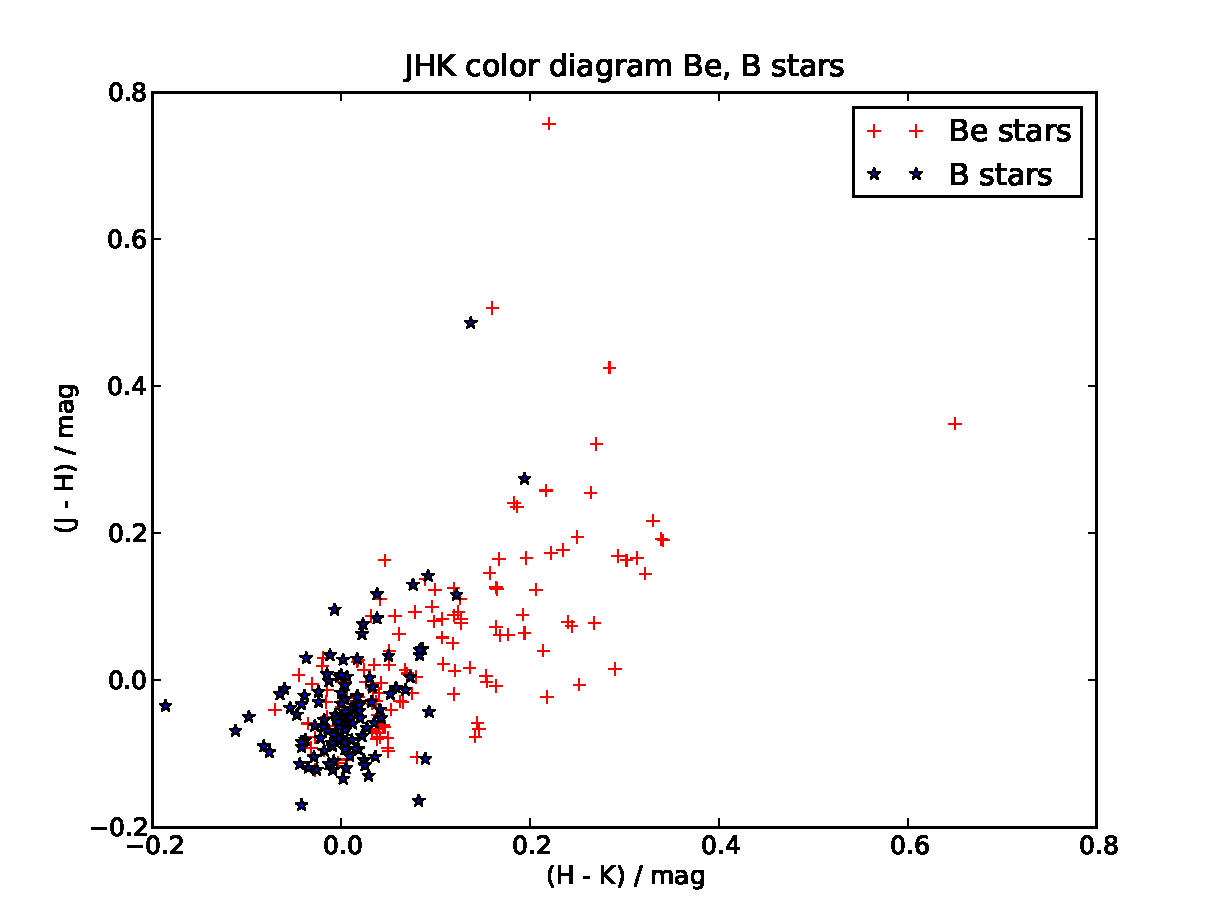
\includegraphics[scale =.6]{jhk_be_b}
        \else
        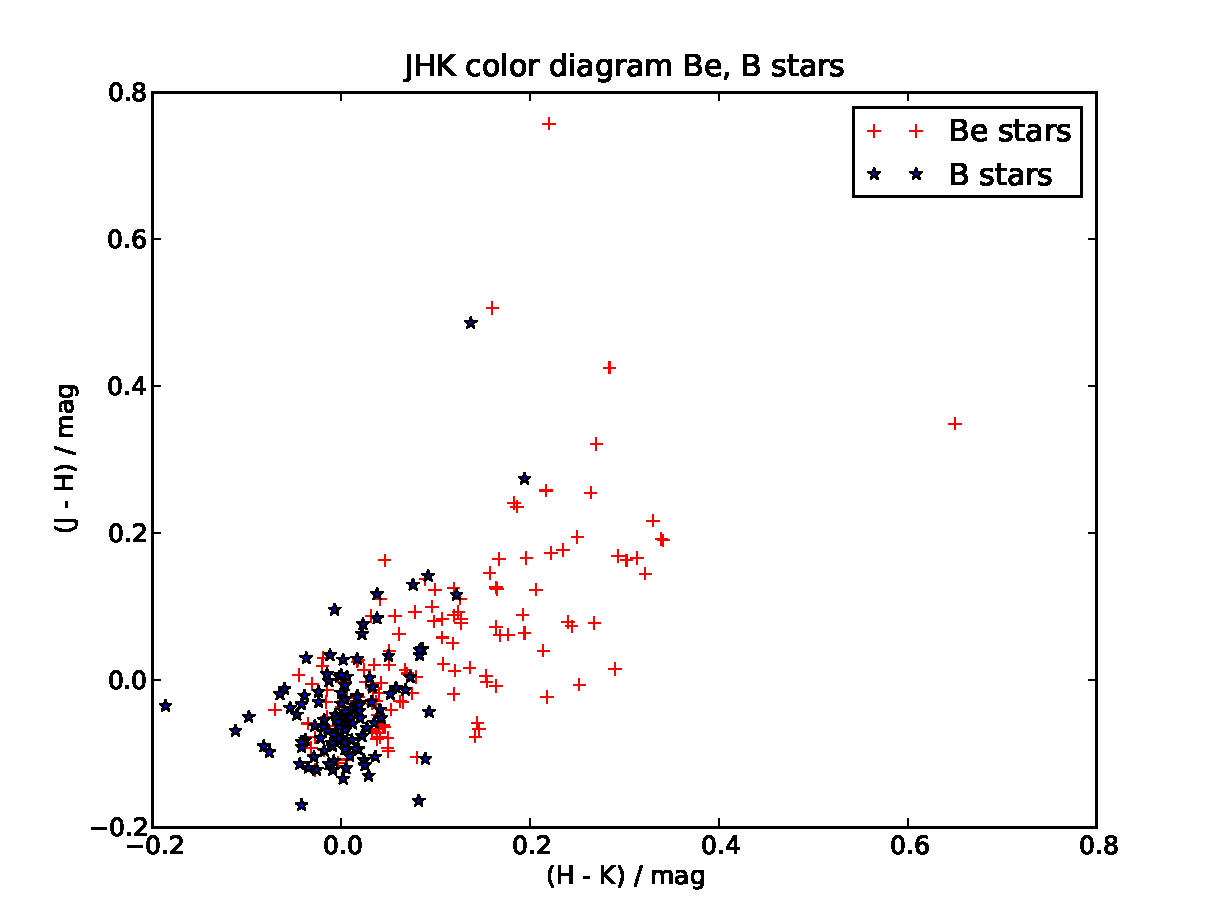
\includegraphics[bb = 92 86 545 742, height=6in]{jhk_be_b}
        \fi
        \caption{Color diagram of confirmed Be stars Vs B stars}
        \label{Figjhk_be_b}
      \end{center}
    \end{figure}

    The uncertainties were computed for each object using propagation
    of error. These errors and depicted on the figure
    \ref{Figjhk_be_b_errors}. Although the uncertainties are
    significant certain trends are presented.

\begin{align*}
  \delta_{(j - h)} = \sqrt{\left(\frac{\partial(j - h) }{\partial
        j}\right)^2\delta_j^2 + \left(\frac{\partial(j - h) }{\partial
        h}\right)^2\delta_h^2} \\
  \frac{\partial(j - h) }{\partial j } = 1,\frac{\partial(j - h)
  }{\partial h } = -1 \\
  \delta_{(j - h)} = \sqrt{\delta_j^2 + \delta_h^2}
\end{align*}


    \begin{figure}[!htbp]
      \begin{center}
        \leavevmode
        \ifpdf
        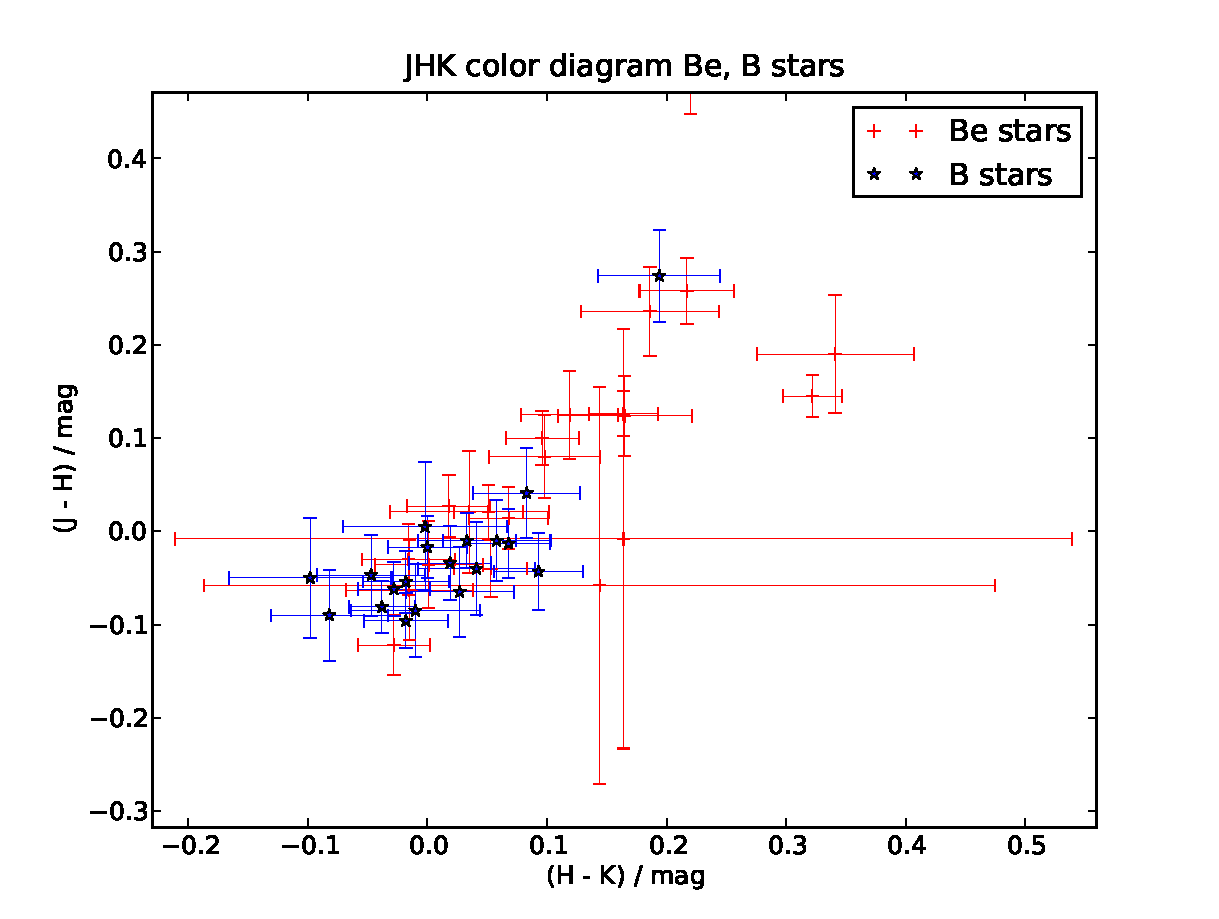
\includegraphics[scale =.6]{jhk_be_b_errors}
        \else
        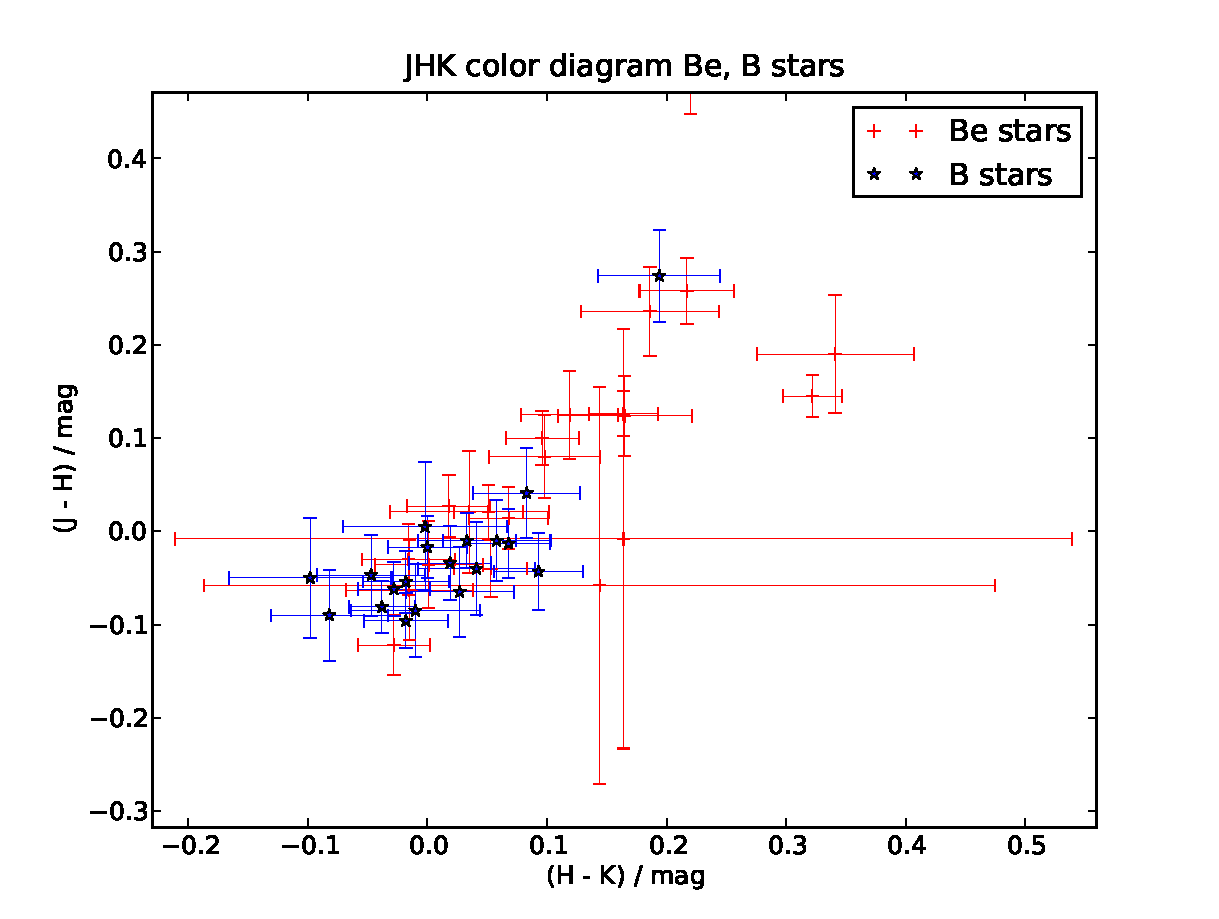
\includegraphics[bb = 92 86 545 742, height=6in]{jhk_be_b_errors}
        \fi
        \caption{Color diagram of confirmed Be stars Vs B stars with errors}
        \label{Figjhk_be_b_errors}
      \end{center}
    \end{figure}

\clearpage


\subsection{Classification}
Data were transformed from original VOTable obtained from Virtual
Observatory tools to arff\footnote{Attribute-Relation File
  Format. Developed by the Machine Learning Project at the Department
  of Computer Science of The University of Waikato.}format used in
Weka Data Mining system. Algorithm C4.5 (J48) was used to perform
actual classification with following result:

\begin{lstlisting}
  Correctly Classified Instances         769               73.0989 %
  Incorrectly Classified Instances       283               26.9011 %
  Kappa statistic                          0.4496
  Mean absolute error                      0.3843
  Root mean squared error                  0.4383
  Relative absolute error                 79.4985 %
  Root relative squared error             89.1648 %
  Total Number of Instances             1052
\end{lstlisting}

As seen on the first row 73 \% from  1052 objects were classified
correctly. More details can be obtained from confusion matrix below.

\begin{lstlisting}
  B   Be   <-- classified as
 304 126 |   B
 157 465 |   Be
\end{lstlisting}

304 of B and 456 of Be stars were classified correctly but 126 of B
and 157 of Be stars were classified incorrectly. In virtue of these
results one should be sceptical if the distinction based only on
photometric properties is significant enough to find relevant new
candidates of Be stars. For this reason more sophisticated (and much
more complicated) approach using spectra analysis was tested.

\section{Spectral Data Mining}

\subsection{Testing Data}
As testing sample the project SEGUE of SDSS were selected. This
contains 178315 spectra in DR7. Following SQL query was used to
generate the list of URL links for individual FITS files. These files
were then download to local sever using wget command.

\begin{lstlisting}
SELECT  objid,dbo.fGetUrlFitsSpectrum(s.specObjID)                                                           
INTO mydb.segue_1                                                                                     
FROM SpecPhotoAll s, platex p                                                                         
WHERE s.specObjID is not null                                                                         
AND s.plateid = p.plateid                                                                             
AND p.programname LIKE 'segue%'                                                                       
AND specClass = 1
\end{lstlisting}

\subsection{Training Data}
The spectra from Ondřejov Observatory were used as training
sample. Files were downloaded using SSA protocol. The SSA server is
not publically aviable, therefore SSH tunneling was used. Two scripts
for this process were created. First to construct the list of SSA
compliant adresses, the second to analyse acquired response in VOTable
format. Then the spectra were downloaded using wget command. The
fuction for constructing the links based on list of the RA, DEC which
were obtained from Hipparcos catalog using the specification of IDs
from Ondřejov's index.

\begin{lstlisting}
def createQuery(data):
    """ From raw data construct ra, dec """
    """ Convert to degrees """
    for line in data:
        ra = ac.AngularCoordinate(line[0:10]).degrees # convert ra to degrees
        dec = ac.AngularCoordinate(line[-13:-1]).degrees # convert dec to degrees
        ra = line[0]
        dec = line[1]
        ssaTemp = 'http://tvoserver/coude/coude.cgi?c=ssac&n=coude_ssa&REQUEST=queryData&POS=<ra>,<dec>&SIZE=1'
        ssaTemp = ssaTemp.replace('<ra>',"%0.3f" % ra)
        ssaTemp = ssaTemp.replace('<dec>',"%0.3f" % dec)
        ssa.append(ssaTemp)
    return ssa
\end{lstlisting}

The script generate the following output. The same process were used
later for obtaining th sample of non Be stars.

\begin{lstlisting}
http://tvoserver/coude/..._ssa&REQUEST=queryData&POS=83.113,-65.582&SIZE=60
http://tvoserver/coude/..._ssa&REQUEST=queryData&POS=162.537,148.333&SIZE=60
http://tvoserver/coude/..._ssa&REQUEST=queryData&POS=19.907,-73.502&SIZE=60
\end{lstlisting}


\subsubsection{Spectra Reduction}
Because spectra from SDSS and Ondřejov Observatory had different
resolution, reduction was needed. First the parameter CD1\_1 (Coordinate
increment per pixel) had to be obtained form FITS file.


\begin{lstlisting}
  In [1]: hdu = pf.open('sdss_test.fit')
  In [2]: hdu[0].header['CD1_1']
  Out[2]: 0.0001 # SDSS spectrum 
  Out[3]: 0.2567 # Onřejov spectrum
\end{lstlisting}

Spectra in SDSS are stored in logarithmic scale thus the value is
computed as $ 10^{CD1\_1} = 1.0002302850208247$. The ratio is then
$CD1\_1_{SDSS}/CD1\_1_{OND} = 3.8964580808433253$. Based on this
computation 4 pixels of Ondřejov's spectra were reduced into
one. There is the critical part of the reduction program:

\begin{lstlisting}
 def convolution(f, g):
    """ Convolve two functions"""
    fg = np.convolve(g,f,'same')
    return fg
 def reduce(x,y,bin):
    """ Reduce bin pixel into 1"""
    size = x.size/bin
    l = 0
    xx = x[:x.size-1:bin]
    yy = list()
    for i in range(0,size):
        s = 0
        for j in range(0,bin):
            s = s + y[l]
            l+=1
        yy.append(s/bin)
    return xx, yy
\end{lstlisting}

Prior to binning pixels convolution with gaussian function was
performed on the spectra. Convolution is defined:

\begin{equation}
  \label{eq:convolution}
 (f * g )(t) \stackrel{\mathrm{def}}{=}\ \int_{-\infty}^{\infty} f(\tau)\, g(t - \tau)\, d\tau
\end{equation}
 
Here it was used in it's dicrete form

\begin{equation}
  \label{eq:discreteConvolution}
  (f * g)[n]\ \stackrel{\mathrm{def}}{=}\ \sum_{m=-\infty}^{\infty} f[m]\, g[n - m]
\end{equation}



The result is on the figure


    \begin{figure}[!htbp]
      \begin{center}
        \leavevmode
        \ifpdf
        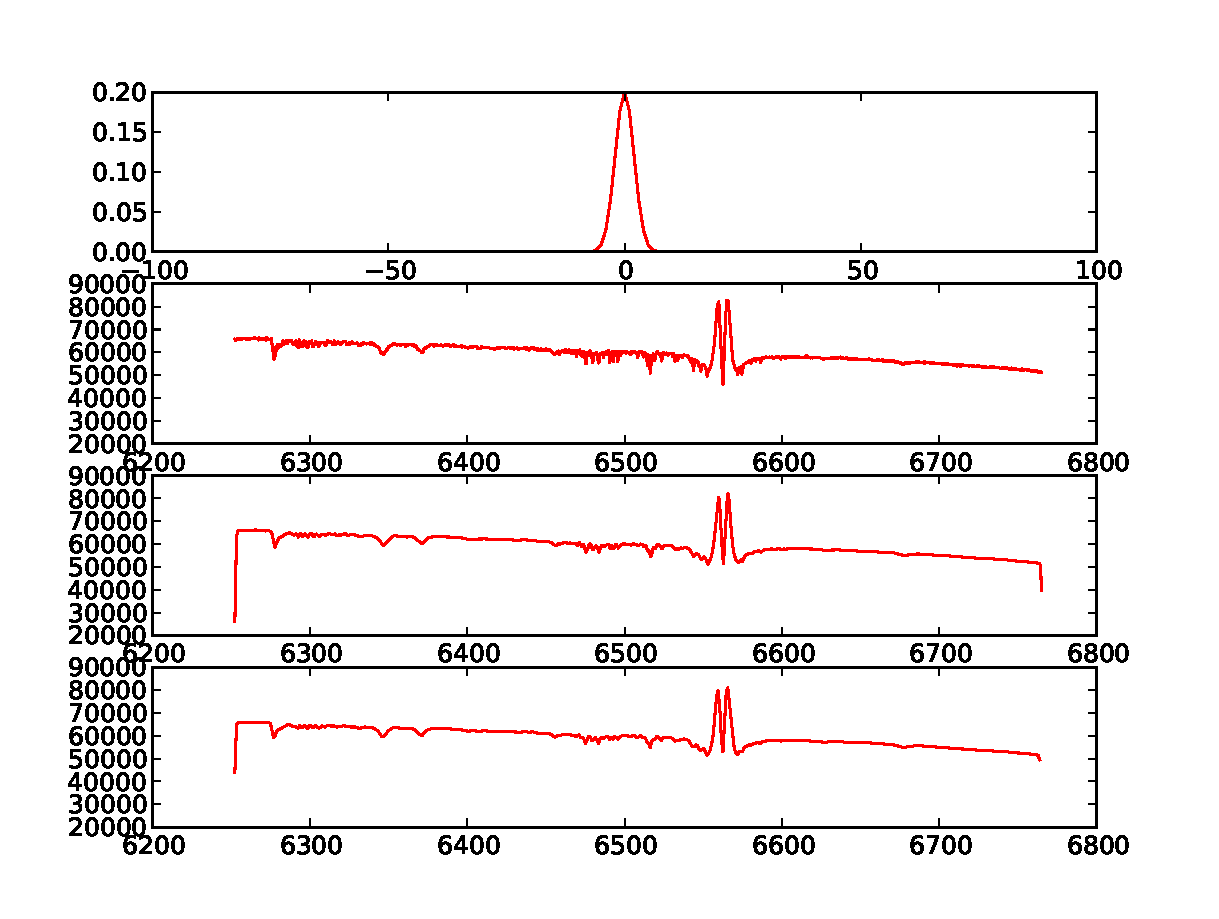
\includegraphics[scale =.8]{convolution}
        \else
        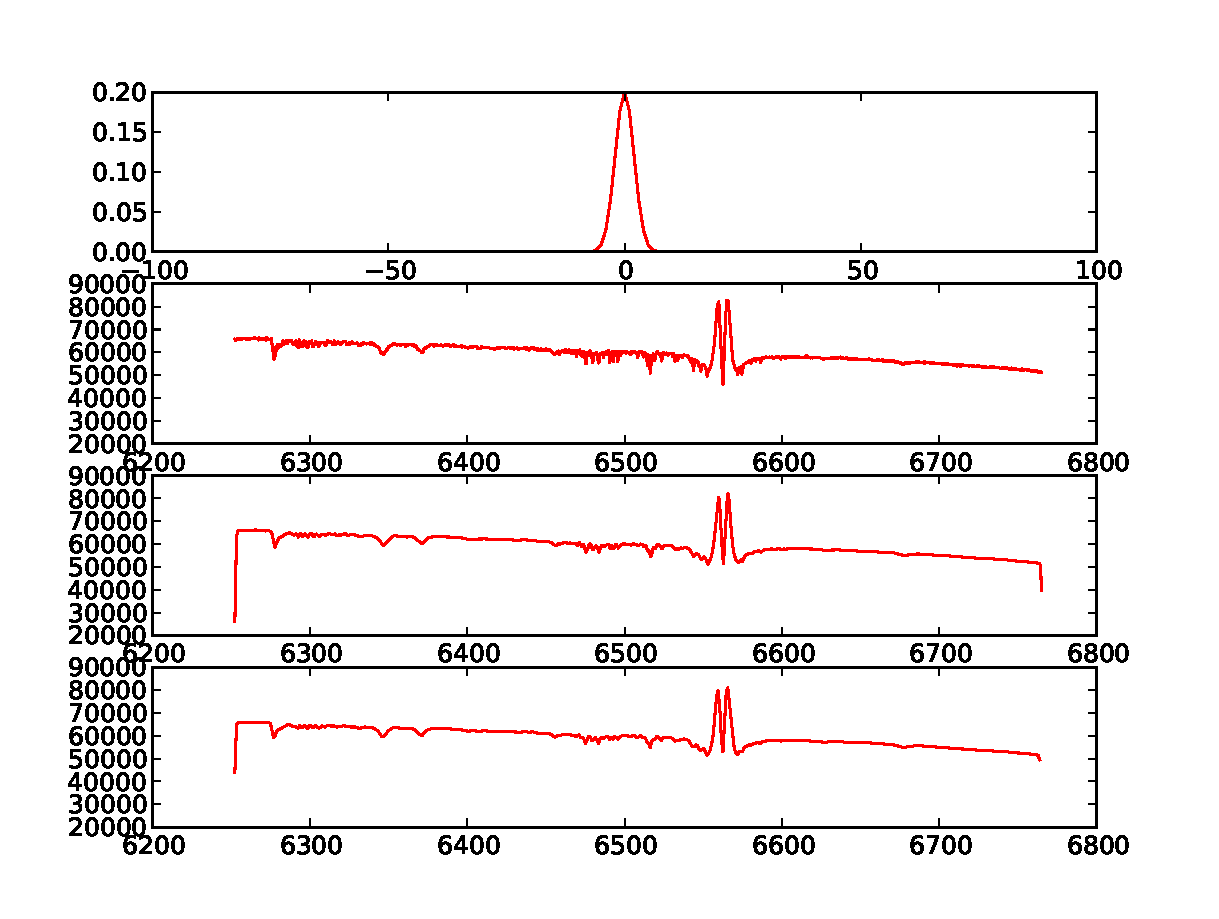
\includegraphics[bb = 92 86 545 742, height=6in]{convolution}
        \fi
        \caption{Reduction of Ondřejov's spectra of the Be star 4
          Hercules. The top figure shows gaussian function used for
          convolution with the structrum, followed by the original
          spectrum then there is a spectrum after convolution with the
          gausian function. The last is the final spectrum after
          reduction.}
        \label{FigReduction}
      \end{center}
    \end{figure}

\clearpage




\subsection{Spectra Lines Characteristics}
As parameters for Data Mining process characteristics value of
H$\alpha$ line were extracted from the spectra. Many possible
characteristics from fitting functions through Wavelets Coefficients
and Eigen Values were discussed with experts. On the end the most
simple approach was used taking the maximum value in the region of
$50\AA$.



\subsubsection{Normalization}
Spectra from SDSS are normalized but the spectra from Ondřejov are
not. Therefore the spectra were devided by it's continuum fit
function. This process ensures the compatibility when comparing the
values for different spectra.


   \begin{figure}[!htbp]
      \begin{center}
        \leavevmode
        \ifpdf
        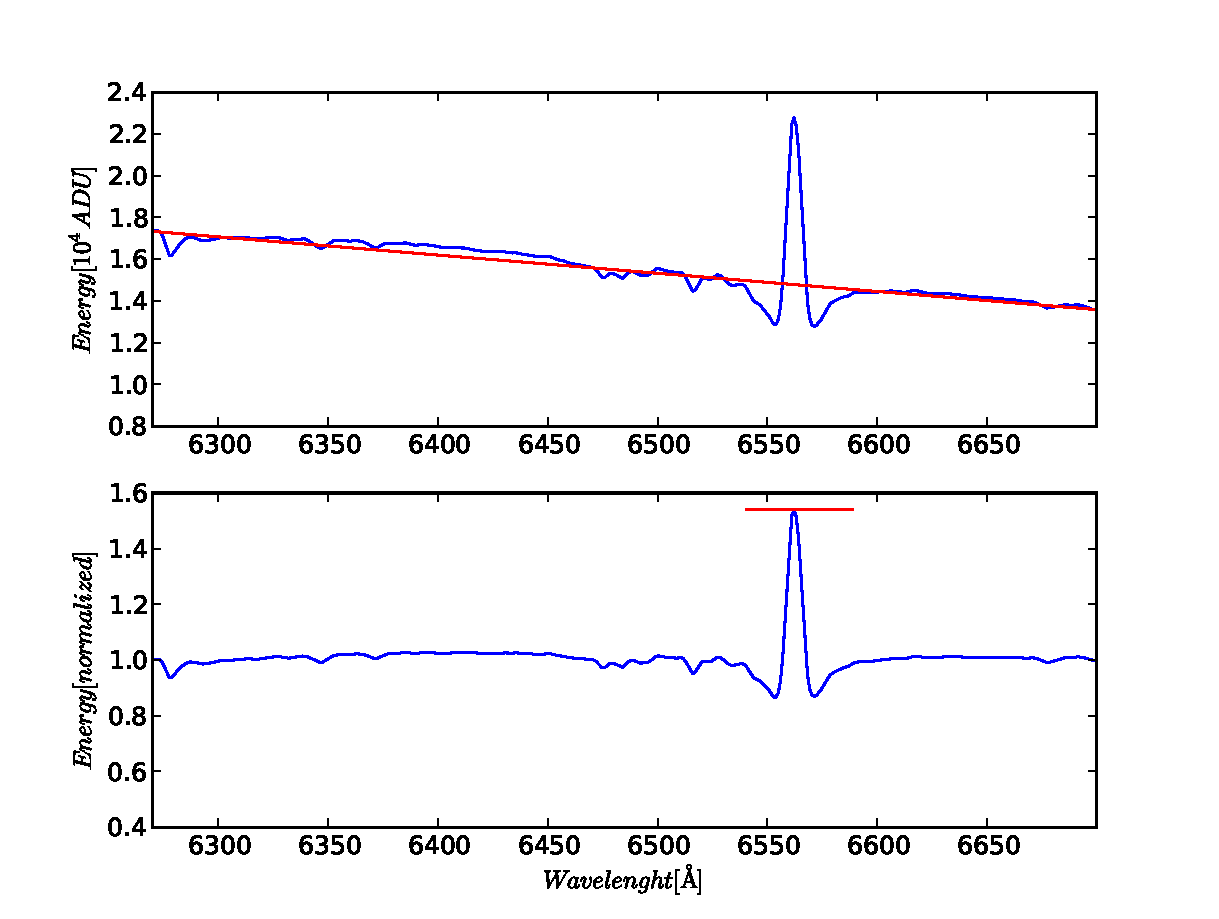
\includegraphics[scale =.8]{beta_cyg_b}
        \else
        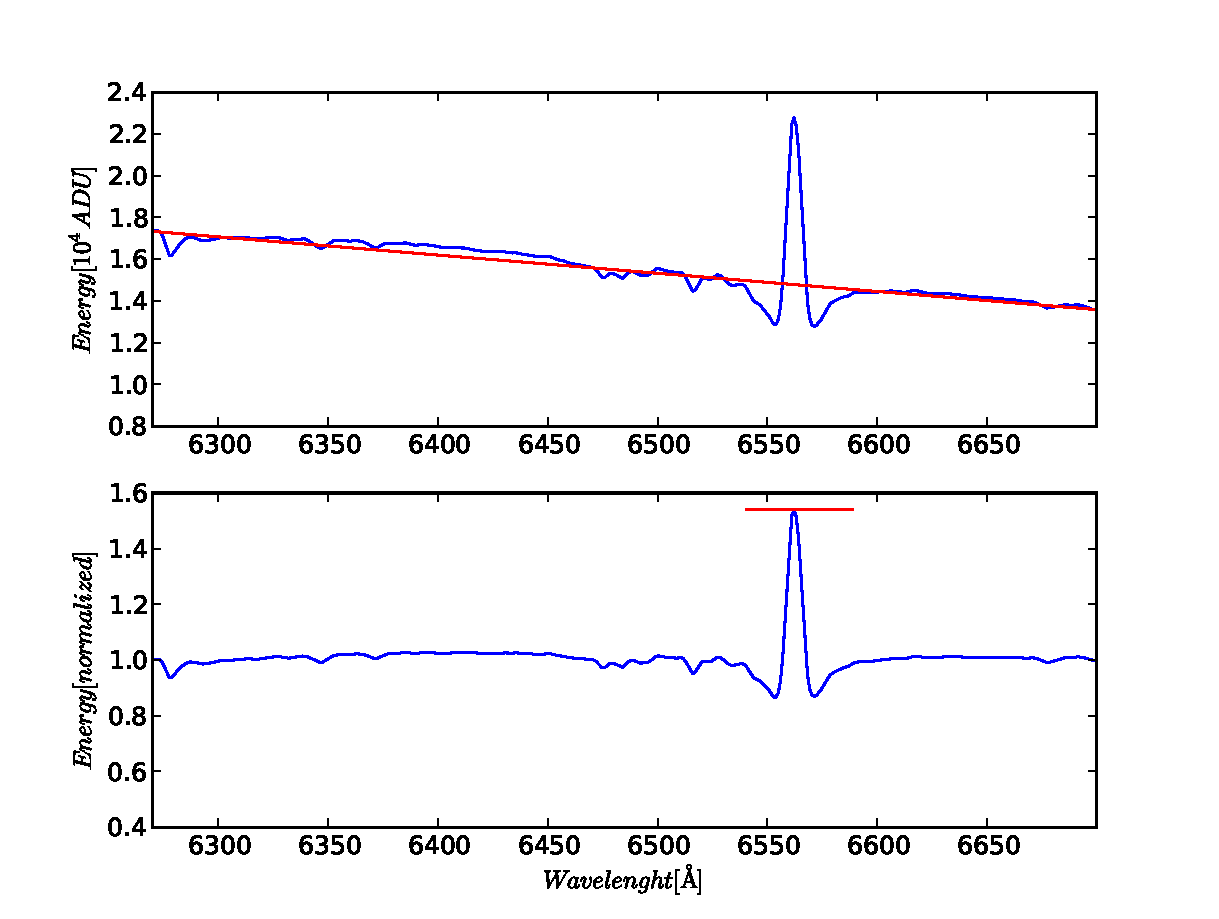
\includegraphics[bb = 92 86 545 742, height=6in]{beta_cyg_b}
        \fi
        \caption{Normalized spectrum of $\beta$ Cygni B (Albireo
          B). The top figure depicts the continuum fit. The bottom
          figure shows the region (width of the red line) used for
          extraction. The position of the line correspond to the
          characteristic value.}
        \label{FigReduction}
      \end{center}
    \end{figure}

\clearpage

The script was written to normalize the spectrum and extract the line
characteristic value. This program also plots the results of the
process as it is shown on previous picture. The function used to
extract the line characteristic value is below.


\begin{lstlisting}
def getMax(x,y,line,range):
    """ Return maximum value of range in the spectrum"""
    xrange = x[(x < line + range) & (x > line - range)]
    yrange = y[(x < line + range) & (x > line - range)] - 1
    maximum = yrange.max()
    minimum = yrange.min()
    if abs(maximum)  > abs(minimum):
        extrem = ( maximum + 1)
        sgn = np.sign(maximum)
    else:
        extrem = (minimum + 1)
        sgn = np.sign(minimum)
    return xrange, extrem, sgn
\end{lstlisting}


